\section{Propósito de la solución}
\label{sec:proposito-solucion}
El propósito de la solución consiste en proveer evaluaciones de desempeño de búsqueda oportunas que permitan a los docentes aplicar acciones correctivas durante el proceso de formación y desarrollo de competencias informacionales en cursos de alfabetización informacional.

Con el módulo propuesto en este trabajo, el docente obtiene una estimación temprana del desempeño del estudiante en el proceso de búsqueda de información, de tal forma que él pueda guiar al estudiante en el proceso. Tal como ilustra la Figura \ref{fig:docente_estudiante}, el estudiante interactúa con el sistema educacional, en este caso NEURONE y la plataforma propuesta a través de técnicas de minería de datos informa al docente de los patrones y predicciones del desempeño de búsqueda del estudiante con el objetivo de ayudar en la toma de decisiones al docente correspondiente para diseñar y planificar de mejor forma la entrega de contenidos hacia el estudiante.

\begin{figure}[H]
	\centering
	%\begin{tikzpicture}[node distance=3.5cm]

%\matrix(m)[matrix of nodes,row sep=3em,column sep=4em,minimum width=2em]{
%	\node[label={Docente}, businessman, minimum size=1.5cm](docente); & \node[label={Estudiante}, charlie, mirrored, monitor,minimum size=1.5cm](estudiante);\\
%};


\node[label={Estudiante},charlie,monitor,minimum size=1.5cm](estudiante);
%motor de busqueda
\node(db)[cylinder, 
        shape border rotate=90, 
        draw,
        minimum height=1.5cm,
        minimum width=2cm,
        shape aspect=.25,
        right=of estudiante] {Motor de búsqueda};

\node[label={Docente},businessman,monitor,mirrored,minimum size=1.5cm,right=of db](docente);


% Draw edges
\draw[arrow] (estudiante) -- (db);
%\draw[arrow] (db) -- (estudiante);
\draw[arrow] (db) -- (docente);

%\draw[->] (B.west) +(0,-1em) coordinate (b1) -- (A.east |- b1);
%\draw[->] (db.west) +(0,-1em) coordinate (b1) -- (A.east |- b1);

\end{tikzpicture}
	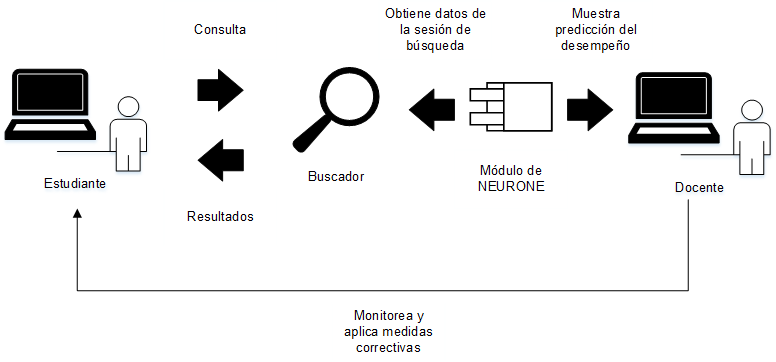
\includegraphics[width=0.9\textwidth]{03_GraphicFiles/monitor.png}
	%\input{03_GraphicFiles/p07.pdf}
	\captionsource{Proceso de búsqueda de información de un estudiante}{\fuentePropia}
	\label{fig:docente_estudiante}
\end{figure}
